%! TEX root = /home/simon/Documents/Dagbok_MPPHS_2020-2021/main.tex
\subsection{Måndag 2020-10-12}

Börjar dra ihop sig till tents nu. Jag borde fortsätta med att recappa integrationsteorin \& kanske börja recappa algebran \&så.


\subsection{Tisdag 2020-10-13}

Fick limes-3a i subben :).

Vi skriver ner en uppdaterad kursplan:
%! TEX root = /home/simon/Documents/Dagbok_MPPHS_2020-2021/main.tex
\begin{table}[H]
    \centering
    \caption{}
    \label{tab:course_plan_2}
    \begin{tabular}{l|l|l|}
         & Year 1 & Year 2 \\ \hline
        LP1 
        & \begin{tabular}[c]{@{}l@{}}
            \textcolor{compulsory}{Learning from data (C)}\\ \textcolor{compulsory}{Quantum mechanics (B)}\\ \textcolor{compulsory}{Experimental physics (A)}\\ Representation theory
        \end{tabular}
        & \begin{tabular}[c]{@{}l@{}} \textcolor{elective}{Standard model \& beyond (B)}\\ Integration theory\\ Commutative algebra
        \end{tabular} \\ \hline
        LP2
        & \begin{tabular}[c]{@{}l@{}}
            \textcolor{compulsory_elective}{Symmetries (A)}\\ \textcolor{compulsory_elective}{Computational physics (D)}
        \end{tabular}
        & \begin{tabular}[c]{@{}l@{}}
            %\textcolor{elective}{String theory (A)}\\
			\textcolor{elective}{High performance computing}\\
            Algebraic geometry\\
            Sannolikhetsteorins grunder?
        \end{tabular} \\ \hline
        LP3
        & \begin{tabular}[c]{@{}l@{}}
            \textcolor{elective}{Gravitation \& cosmology (A)}\\ Advanced differential calculus
        \end{tabular} &  \\ \hline
        LP4
        & \begin{tabular}[c]{@{}l@{}}
            \textcolor{elective}{Quantum field theory (B)}\\ Vetenskapshistoria (LA)\\ Complex analysis in several variables
        \end{tabular} 
        & \begin{tabular}[c]{@{}l@{}}
            Distributionsteori?
        \end{tabular} \\ \hline
    \end{tabular}
\end{table}


\bigskip

Hade möte med Thomas Bäckdahl nu \& det kändes bra.
Han sa att de mest relevanta kurserna var GR \& diffkalkylen, vilket känns bra nu när jag skippar strängen.
Han sa till \& med att HPC:n nog var fett användbar så känns inte fel att jag tar den nu.
Sammanfattningsvis är idén att jag ska \enquote{undersöka vad som krävs av en rumstid för existens av lösningar till massiva Dirac-ekvationen med hjälp av xAct (\& liknande?) för att hitta irreducibla dekompositioner. Detta baseras på artikeln \enquote{second order symmetry operators}}.

Jag kollade lite \&så på det administrativa \& det verkar inte som att det finns några deadlines. + att Ludde hade inte gjort ngt offeciellt än heller. När det börjar dra ihop sig ska jag skicka in en blankett till
\begin{itemize}
	\item masteransvarig
	\item examinator
	\item instutitionen (MV).
\end{itemize}
Men den mesta infon finns i \verb|Föreskrifter för masterexamensarbeten_2016.pdf|. Annars tänker jag att det jag har att göra nu framöver är att läsa kap.\ 13 i Walds General Relativity som Thomas rekomenderade.


\subsection{torsdag 2020-10-15}

Jag lade hela dagen på att få till ett najjs synthwavetema på vscode. Det blev jättebodgeit \& fungerar bara när jag kör vscode som root. Men det blev fett spaceat
\begin{figure}[H]
	\centering
	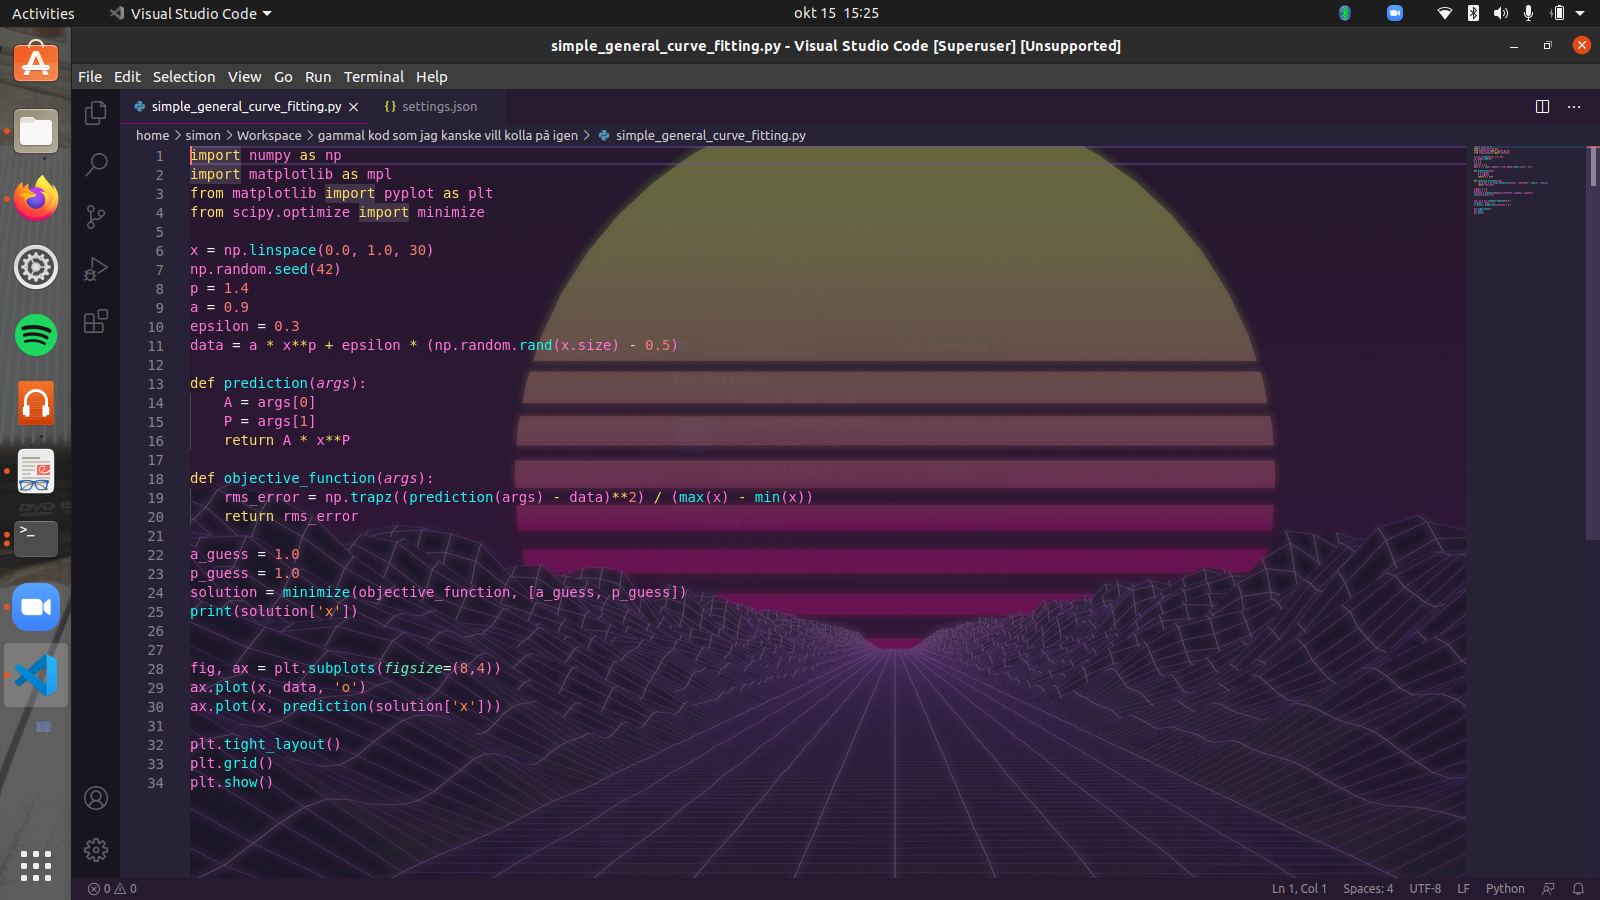
\includegraphics[width=1.0\textwidth]{pics/synthwave_vscode.png}
\end{figure}

Träffade Pontus sen på eftermiddagen \&så, det var fett mysigt. Han berättade bland annat att dom flesta hissar fungerar med relän. det finns alltså ingen mjukvara utan allt är i princip mekaniskt! Även om detta är lite förvånande kan jag se en stor fördel med varför man inte skulle vilja ändå. Det hade inte varit supernajjs om terrorister kunnat hacka hissar.


\subsection{Fredag 2020-10-16}

Lämnade in standardmodellen idag. Hoppas allt e godkännt nu, jag har bodgeat lite med dom två sista inlämningarna. Men om det är det så har jag bara massa integrationsteori \& algebra framför mig. Vilket kommer bli fett hype!

En idé som jag snackade med Eric \& Kevin om idag på lunchen är problemet med om man ska köpa byxor nya eller begagnade.
Om jag köper ett par nya har dom ju inget slitage än så naivt borde man ju tänka att väntevärdet för hur länge dom kommer hålla är större än för ett par begagnade byxor.
Men man måste ju \&så tänka på att om man köper ett par begagnade så är sannolikhetsfördelningen betingad på att dom hållt dittills.
Om $T$ är en slumpvariabel som beskriver hur lång tid ett par byxor håller, så är sannolikheten att de håller en tid $t$, givet att de redan hållt en tid $t_0$, enligt definitionen av betingad sannolikhet
\begin{align}
	P(t \leq T \mid t_0 \leq T) = \frac{P(t \leq T \qq{\&} t_0 \leq T)}{P(t_0 \leq T)} = \begin{cases}
	\frac{P(t \leq T)}{P(t_0 \leq T)} &\qq{om $t_0 \leq t$}\\
	1 &\qq{om $t < t_0$}
	\end{cases}.
\end{align}
Alltså kan man bara ta samma pdf, sätta allt innan $t_0$ till $0$, \& normera.
Vi konstaterade att det kan vara svårt att hitta data på byxor. Eric föreslog att man kanske kan hitta data på hårdiskar.

 
